% Template for a Computer Science Tripos Part II project dissertation
\documentclass[12pt,a4paper,oneside,openright]{report}

\usepackage{amsmath, amsthm, amssymb}
\usepackage{array}
\usepackage{color}
\usepackage{docmute}   % only needed to allow inclusion of proposal.tex
\usepackage[margin=15mm]{geometry}  % adjusts page layout
\usepackage{graphicx}  % allows inclusion of PDF, PNG and JPG images
\usepackage[pdfborder={0 0 0}]{hyperref}    % turns references into hyperlinks
\usepackage{pdfpages}
\usepackage{verbatim}


\newcolumntype{C}{>{{}}c<{{}}}

\setlength{\parindent}{0ex}

\clubpenalty1000%
\raggedbottom                           % try to avoid widows and orphans
\renewcommand{\baselinestretch}{1.1}    % adjust line spacing to make readable
\sloppy
\widowpenalty1000%

\begin{document}
\bibliographystyle{plain}

%%%%%%%%%%%%%%%%%%%%%%%%%%%%%%%%%%%%%%%%%%%%%%%%%%%%%%%%%%%%%%%%%%%%%%%%
% Title

{\let\cleardoublepage}

\rightline{\LARGE \textbf{Marius Latinis}}

\vspace*{60mm}
\begin{center}
\Huge
\textbf{Bus Arrival Time Prediction} \\[5mm]
Computer Science Tripos -- Part II \\[5mm]
Christ's College \\[5mm]
\today  % today's date
\end{center}
\newpage

%%%%%%%%%%%%%%%%%%%%%%%%%%%%%%%%%%%%%%%%%%%%%%%%%%%%%%%%%%%%%%%%%%%%%%%%%%%%%%
% Proforma, table of contents and list of figures

\pagestyle{empty}

\chapter*{Proforma}

{\large
\begin{tabular}{ll}
\textcolor{blue}{Name}: & \bf Marius Latinis                        \\
\textcolor{blue}{College}:            & \bf Christ's College                     \\
\textcolor{blue}{Project Title}:      & \bf Bus Arrival Time Prediction \\
\textcolor{blue}{Examination}:        & \bf Computer Science Tripos -- Part II, July 2017  \\
\textcolor{blue}{Word Count}:         & \bf \textcolor{red}{TODO(ml693): figure out} \\
\textcolor{blue}{Project Originator}: & \bf Dr Richard Mortier \\
\textcolor{blue}{Supervisor}:         & \bf Dr Richard Mortier \\ 
\end{tabular}
}
\stepcounter{footnote}


\section*{Original Aims of the Project}

Implement an algorithm which given the most recent GPS data predicts
when the bus will arrive at the future stops. Evaluate the algorithm
and show that on average it predicts with error less than 80s.

\section*{Work Completed}

All that has been completed appears in this dissertation.

\section*{Special Difficulties}

None
 
\section*{Declaration}

I, Marius Latinis of Christ's College, being a candidate for Part II of the Computer
Science Tripos, hereby declare that this dissertation and the work described 
in it are my own work, unaided except as may be specified below,
and that the dissertation does not contain material that has already been used to any substantial extent for a comparable purpose.

\bigskip
\leftline{Signed [signature]}

\medskip
\leftline{Date \today}

\tableofcontents

%%%%%%%%%%%%%%%%%%%%%%%%%%%%%%%%%%%%%%%%%%%%%%%%%%%%%%%%%%%%%%%%%%%%%%%
% now for the chapters

\pagestyle{plain}








\chapter{Introduction}

\section*{Motivation}

In European countries public buses is a popular form of transportation. However,
buses often arrive later than the timetable announces. Therefore, the project aims
to build an algorithm which accuratelly predicts the bus arrival times based on the
most recent GPS data.

\section*{Actual Problem Overview}

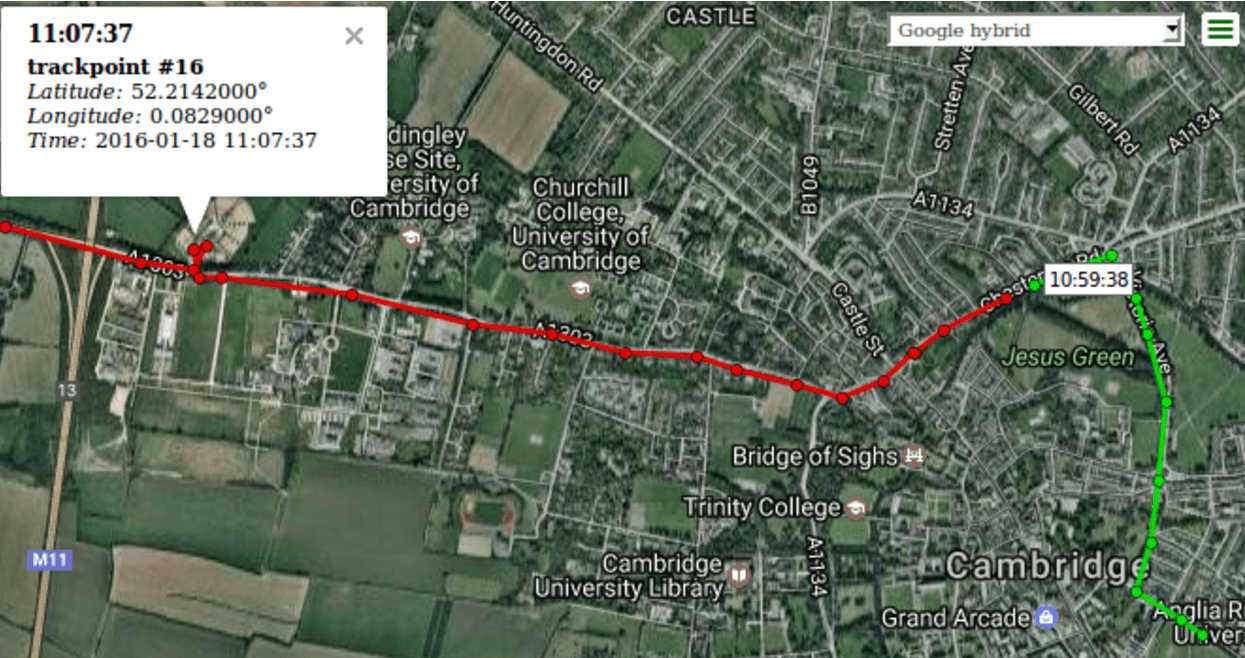
\includegraphics[width=\textwidth]{figs/problem_overview.png} \\

The most recent GPS data (represented by green in the diagram above) shows 
where the bus has travelled up to now. The future data (represented by red)
is not known during the prediction phase. My goal is to predict the future
data given the present data. \\

In this specific example I want to predict when the bus will reach Madingley Park 
starting from Chesterton Road. One can see it takes about 8 min. (10:59--11:07)
to travel such distance.





\chapter{Preparation}

\section*{Starting Point}

A company named Vix is sending real-time GPS data to Cambridge servers. The GPS
data covers East-England bus companies \textcolor{red}{TODO(ml693): which???}. Cambridge
converts the binary GPS data into a human readable JSON format. To start with,
I was given 2 months JSON data (June and July 2016). That was the starting
point data. \\

I started coding completely from scratch.

\section*{Preliminary Work}
\textcolor{red}{TODO(ml693): put something here}






\chapter{Implementation}

\section{Data Preprocessing}

Below is the starting point input data example: \\
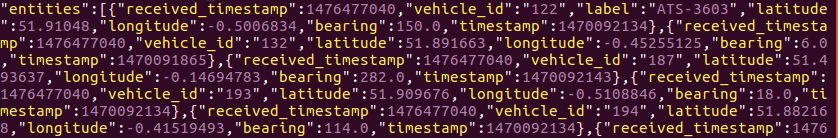
\includegraphics[width=\textwidth]{figs/starting_data.png} \\

One file contains a single snapshot of all buses, 
with one entry per bus. An entry such as:

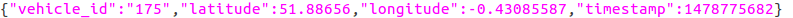
\includegraphics[width=\textwidth]{figs/entry.png} \\

means that a vehicle nr. $56$ was at geographical position
$(51.88010, -0.42051104)$ on the $1$st August $2016$, GMT time
$22$:$51$:$05$\footnote{calculated from timestamp field}. \\

A new snapshot file arrives once in $30$s. The data preprocessing part
takes all input files and converts them into another format: \\

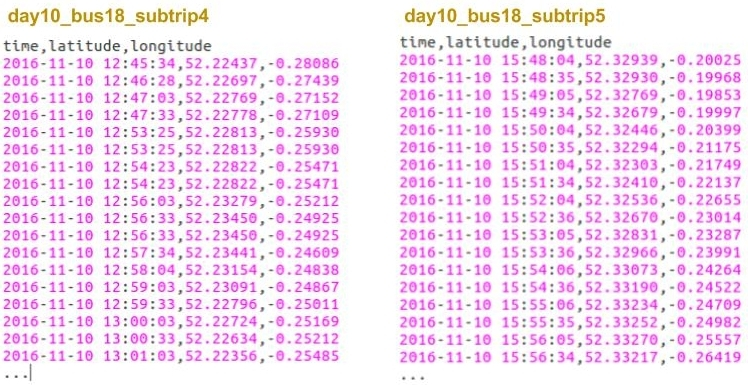
\includegraphics[width=\textwidth]{figs/converted_format.jpg} \\

At the end I have a file for each trip made by one bus in one
day\footnote{note that a bus on a particurlar day could have made
multiple trips}. \\

\section{Route Detection Algorithm}

\subsection{Why an Algorithm is Needed}

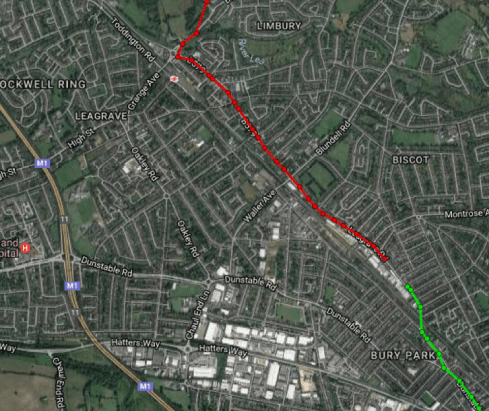
\includegraphics[scale=0.8]{figs/route_detector.png} \\

The GPS points indicated in green show how the bus has moved so far.
The red points show where the bus will travel in the future,
a path I do not know yet. Predicting when the bus will arrive at the stop
requires knowing \textbf{where} a bus will travel next. How? \\

\textbf{Approach Using Static Data} \\

A standard way to find out where the bus will travel next is to know its 
route in advance. Some GPS entries contain additional fields,
such as a \textbf{label}: \\

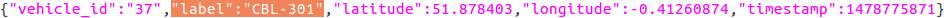
\includegraphics[width=\textwidth, scale=1.2]{figs/labelled_entry.png} \\

An extra field \textbf{label} names the route a bus follows. Auxiliary
data might indicate what route the label \textbf{ATS-3603} corresponds to.
One can then look at the route and determine a sequence of stops 
a bus will visit next. \\

Unfortunately, this approach has drawbacks:

\begin{itemize}
\item Not all entries contain auxiliary fields. After all, the GPS device on the
actual vehicle is responsible only for providing the latitude and longitude
coordinates, not the route a bus follows.

\item Good static data to infer routes based on additional fields is not 
straightforward to find. Field values might not match
(e.g. a route named \textbf{SW-4} in the real-time data is actually \textbf{SWX-4}). Buses are often changing routes\footnote{a
vehicle is unlikely to follow the same route every day} and data does not always
indicate that.

\item The static data only shows the sequence of bus stops, not a detailed
sequence of streets a bus will follow. It is much better to know an actual
path for accurate arrival time prediction.
\end{itemize}

\textbf{New Approach Overview} \\

To overcome the static data limitations, I propose a new way to infer the
route a vehicle is following. I will align a sub-trip how the bus has moved
so far with a historical path for which the route is known. The path aligning
best to the current sub-trip will be used to predict where a bus travels next.
To perform the alignment, I constructed an algorithm\footnote{from now on referred to as a boolean predicate} that can tell whether one sequence of GPS points follows another.

\subsection{$FollowsPath$ Predicate Definition}

I define a predicate $FollowsPath(sub$-$trip, path)$ to be true iff a $sub$-$trip$
follows a $path$: \\

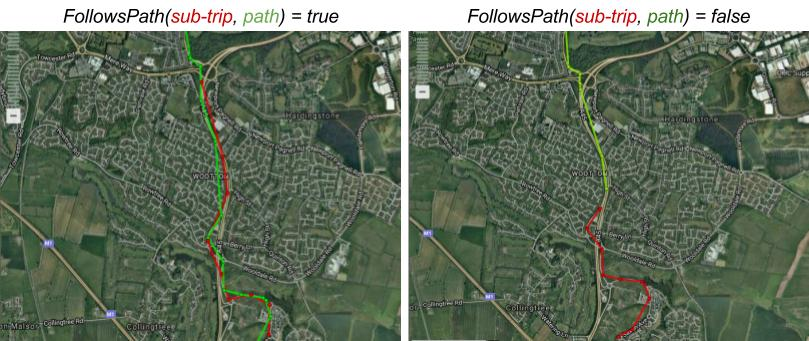
\includegraphics[width=\textwidth, scale=1.2]{figs/follows_path.jpg} \\

Two pictures show when I want the predicate to return true and when false.
For the first example, the predicate returns true because it is intuitively
clear that a red sub-trip follows a blue path. In the second example, the
output is false, as the two GPS sequences do not intersect at all.

\newpage

\subsection{$FollowsPath$ Predicate Implementation}

Firstly, consider the case when a \textcolor{red}{sub- trip's} GPS points
$(\textcolor{red}{P_0}, \textcolor{red}{P_1}, ..., \textcolor{red}{P_{n-1}})$
\textbf{exactly} follow another \textcolor{blue}{path}: \\

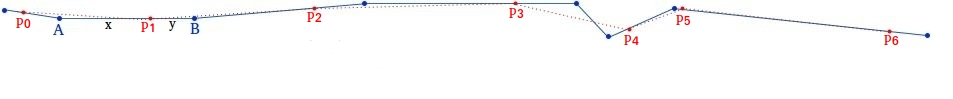
\includegraphics[width=\textwidth]{figs/follows_exactly.jpg}

Each point $P_i$ is on some segment of another trip's path.
For example, $P_1$ is on the segment $AB$.
Let $x = |AP_1|$ and $y = |P_1B|$. Then the
error\footnote{error function takes a point and a segment as an input} function
defined as \\

\begin{centering}
$err(P_1, AB) = \frac{x + y}{|AB|} - 1$ \\
\end{centering}

\:
\:
\:

equals $0$. For each point $P_i$, I find a segment $S_{P_i}$ such that
$err(P_i, S_{P_i})$ is minimised. The $FollowsPath$ predicate returns true
iff

\begin{centering}
    $S = \sum_{i=0}^{n-1} err(P_i, S_{P_i}) < n\epsilon$ \\
\end{centering}

\:
\:
\:

for a suitably chosen threshold value $\epsilon$\footnote{$\epsilon = 0.3$
is one choice}. \\

Note that $S = 0$ when a \textcolor{red}{sub-trip} follows a
\textcolor{blue}{path} exactly. Therefore, in this case, the $FollowsPath$
predicate returns true, which is what I want. \\

The case when a \textcolor{red}{sub-trip} does follow a
\textcolor{blue}{path}, but not exactly (the real world situation), 
is illustrated in the following picture: \\

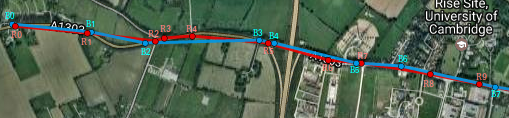
\includegraphics[width=\textwidth]{figs/follows_roughly.png}

In this example I am aligning a \textcolor{red}{sub-trip}
$(\textcolor{red}{R_0}, ..., \textcolor{red}{R_9})$ with a \textcolor{blue}{path}
$(\textcolor{cyan}{B_0}, ..., \textcolor{cyan}{B_7}, ...)$.
The computation of $S$ proceeds as follows:
\[
\setlength\arraycolsep{0pt}
\begin{array}{ *{7}{cC} c }
 S &=& err(\textcolor{red}{R_0}, \textcolor{cyan}{{B_0}{B_1}}) &+& 
       err(\textcolor{red}{R_1}, \textcolor{cyan}{{B_0}{B_1}}) &+& 
       err(\textcolor{red}{R_2}, \textcolor{cyan}{{B_2}{B_3}}) &+& 
       err(\textcolor{red}{R_3}, \textcolor{cyan}{{B_2}{B_3}}) &+& 
       err(\textcolor{red}{R_4}, \textcolor{cyan}{{B_2}{B_3}}) &+  \\
   & & err(\textcolor{red}{R_5}, \textcolor{cyan}{{B_3}{B_4}}) &+& 
       err(\textcolor{red}{R_6}, \textcolor{cyan}{{B_4}{B_5}}) &+& 
       err(\textcolor{red}{R_7}, \textcolor{cyan}{{B_5}{B_6}}) &+& 
       err(\textcolor{red}{R_8}, \textcolor{cyan}{{B_6}{B_7}}) &+&
       err(\textcolor{red}{R_9}, \textcolor{cyan}{{B_6}{B_7}}) &   \\
   &=& (1.0294 - 1)  &+& (1.0300 - 1) &+& (1.0021 - 1)  &+& (1.0730 - 1)  &+& 
       (1.0208 - 1)   &+  \\ 
   & & (1.0714 - 1)  &+& (1.0286 - 1)  &+& (1.0158 - 1)  &+&  (1.0126 - 1)  &+& 
       (1.0125 - 1)   &<& 10 \cdot 0.3 =& n\epsilon
\end{array}
\]

and the predicate again returns true, as desired. \\

Finally, when a sub-trip does not follow a path,
triangle inequality will ensure large values of
$err(P_i, S_{P_i})$\footnote{$err(P_i, S_{P_i}) = \frac{x_i + y_i}{|S_{P_i}|} - 1
\gg (1 + \epsilon) - 1 = \epsilon \implies S \gg n\epsilon$},
thus the sum $S$ will exceed $n\epsilon$, and the predicate will return false. \\

The practical evidence that $FollowsPath$ predicate works is shown in the 
evaluation section.

\newpage

\section{Arrival Time Prediction}

\subsection{Basic Idea}

The $FollowsPath$ predicate allows to detect the route a bus is following.
The route tells the next stops a bus will visit. This section shows how to
predict the arrival time to each future bus stop. \\

Historical trips (which follow the same route) are used to make a prediction:

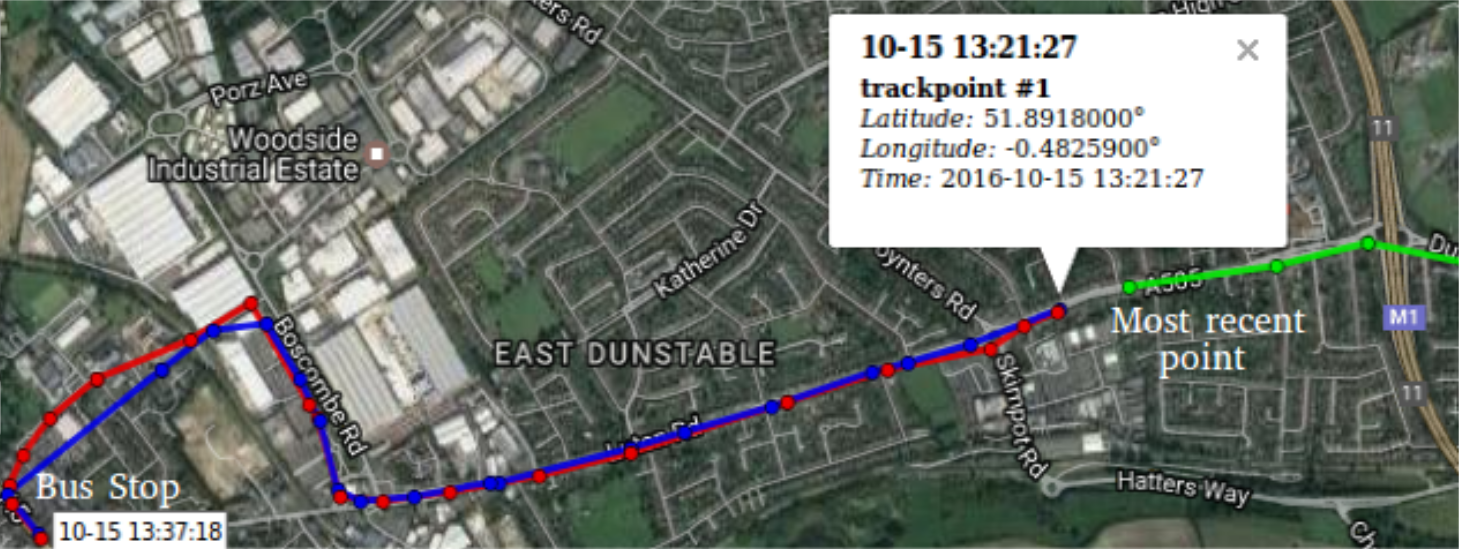
\includegraphics[width=\textwidth]{figs/future_stop.png} \\

In the picture above 2 example historical sub-trips (\textcolor{blue}{blue}
and \textcolor{red}{red}) are shown.
Both of them start where the vehicle currently located is (indicated
by the most recent green point). Both of them represent the history how past
vehicles travelled until the bus stop. I compute the duration how long it
took for each historical trip to reach the bus stop. Knowing multiple duration
values I return the median as the predicted arrival time.

\subsection{Optimisation Nr. 1}

If in the historical trips set certain trips have \textbf{just} travelled along
the same route (e.g. in the last $30$min.), I predict the median time just from
those recent trips. Otherwise, the basic approach is used.

\subsection{Optimisation Nr. 2}

Suppose the most recent data

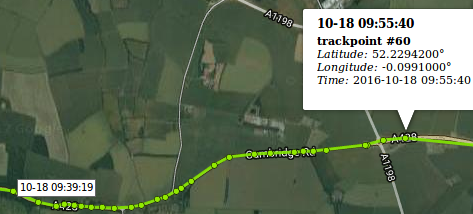
\includegraphics[scale = 0.7]{figs/recent_trip.png} \\

shows the distance a bus has travelled in the last $16$ minutes. Certain historical
trips

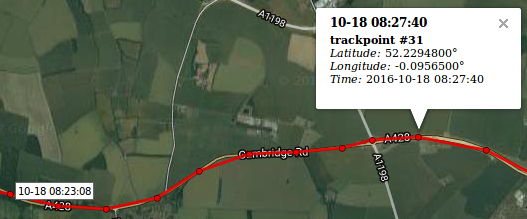
\includegraphics[scale = 0.7]{figs/inaccurate_historical.png} \\

have travelled the same distance in a very different amount of 
time\footnote{this could have happened due different traffic congestion level
in a different time of the day} (e.g. $4$ min.). Predicting arrival time using
these historical trips can be misleading. Hence I filter out such trips.
I.E. I take only those historical trips into account that have travelled the same
distance in roughly the same amount of time\footnote{up to 30sec. difference
is allowed}. \\

Optimisations are tested in the evaluation section.



\section{Real-time System}


\textcolor{red}{TODO(ml693): finish implementing it}



\chapter{Evaluation}

\section{Overview}
\newpage

\section{Route Detection Evaluation}

I break the evaluation of route detection algorithm into multiple steps.

\subsection{Sensitivity Score}

The first step is to check whether the 
$FollowsPath(sub$-$trip, path)$ predicate returns $true$ when the $sub$-$trip$
indeed follows the $path$. \\

I have 10 routes, each route has an associated path,
\textcolor{red}{one} of which is shown 
below\footnote{Arundel Road on the top left is the first bus stop here}: \\
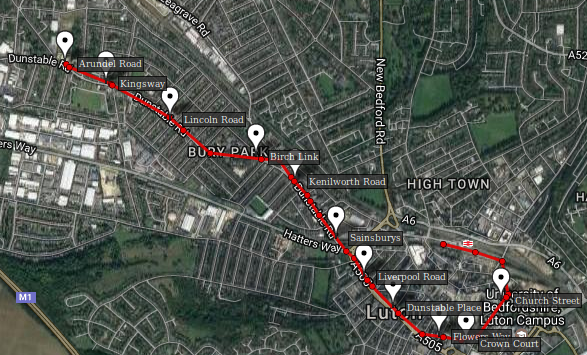
\includegraphics[scale = 0.7]{figs/full_route.png} \\

I have a set of trips $T_p$ that actually follow the path $p$.
For each trip $t \in T_p$ I take a \textcolor{blue}{$sub$-$trip$} \\
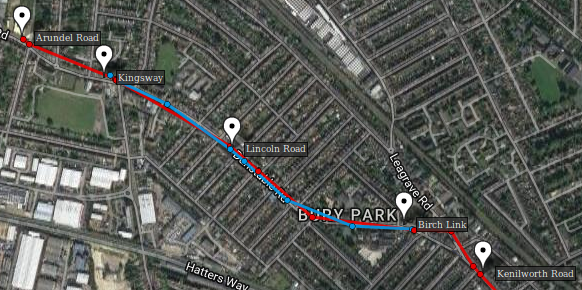
\includegraphics[scale = 0.7]{figs/stop1.png} \\

and check whether the
$FollowsPath($\textcolor{blue}{$sub$-$trip$}, \textcolor{red}{$path$}$)$ 
predicate returns true or false. \\

If the \textcolor{blue}{$sub$-$trip$} does \textbf{not} start from the 
first stop, the $FollowsPath$ predicate has $100\%$ success rate 
for each route. \\

\newpage

If the \textcolor{blue}{$sub$-$trip$} starts from the first stop,
the success rate drops significantly (and becomes unpredictable) due to 
the reason illustrated in the following picture: \\

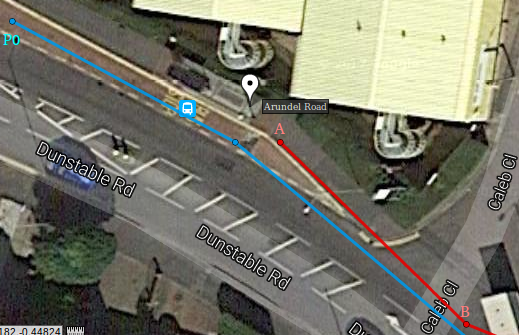
\includegraphics[scale = 0.7]{figs/stop0.png} \\

One can see that $err(P_0, S_{P_0}) = \frac{|{P_0}A| + |{P_0}B|}{|AB|} - 1$
might become large. In fact, accumulated errors for the first few points (when the bus is not on any route yet) are so large the total sum exceeds $n\epsilon$ even if errors for the next points are small. \\

The conclusion is thus to discard the first few GPS points and start using
$FollowsPath$ predicate after the bus has moved for a while and is following 
some route.

\chapter{Conclusion}

I implemented an algorithm which gives sensible prediction results. The
algorithm itself is simple, thus anyone coming after me to improve the
system should not have trouble read and understand what has been done so far. \\

If started again, I would have worked in exactly the same way.


%%%%%%%%%%%%%%%%%%%%%%%%%%%%%%%%%%%%%%%%%%%%%%%%%%%%%%%%%%%%%%%%%%%%%
% the bibliography
\addcontentsline{toc}{chapter}{Bibliography}
\bibliography{refs}

%%%%%%%%%%%%%%%%%%%%%%%%%%%%%%%%%%%%%%%%%%%%%%%%%%%%%%%%%%%%%%%%%%%%%
% the appendices
\appendix

\chapter{Links}

\begin{enumerate}
\item Dynamic time warping is an algorithm for measuring similarity between
two temporal sequences which may vary in speed. For instance, similarities in
walking could be detected using DTW, even if one person was walking faster than
another. I used DTW algorithm as a core part to implement my $FollowsPath$
predicate, with $err$ function being used instead of a regular distance function 
$d(x, y)$.
For more info look at

\textcolor{blue}{\url{https://en.wikipedia.org/wiki/Dynamic_time_warping}}

\item Arrival time prediction problem has been studied before. Two papers that
I read and compared my project with are:

\begin{itemize}

\item Bin Yu, William H.K. Lam, Mei Lam Tam: Bus arrival time prediction at
bus stop with multiple routes 

\textcolor{blue}{\url{http://www.sciencedirect.com/science/article/pii/S0968090X11000155}}

\item Pengfei Zhou, Yuanqing Zheng, Mo Li: How Long to Wait? Predicting Bus Arrival Time with Mobile Phone based Participatory Sensing

\textcolor{blue}{\url{http://www.ntu.edu.sg/home/limo/papers/sys012fp.pdf}}

\end{itemize}

\item Project code can be found at: 

\textcolor{blue}{\url{https://github.com/ml693/bus}}


\end{enumerate}

\chapter{Detailed Evaluation Results}

\chapter{Project Proposal}
(see next page)

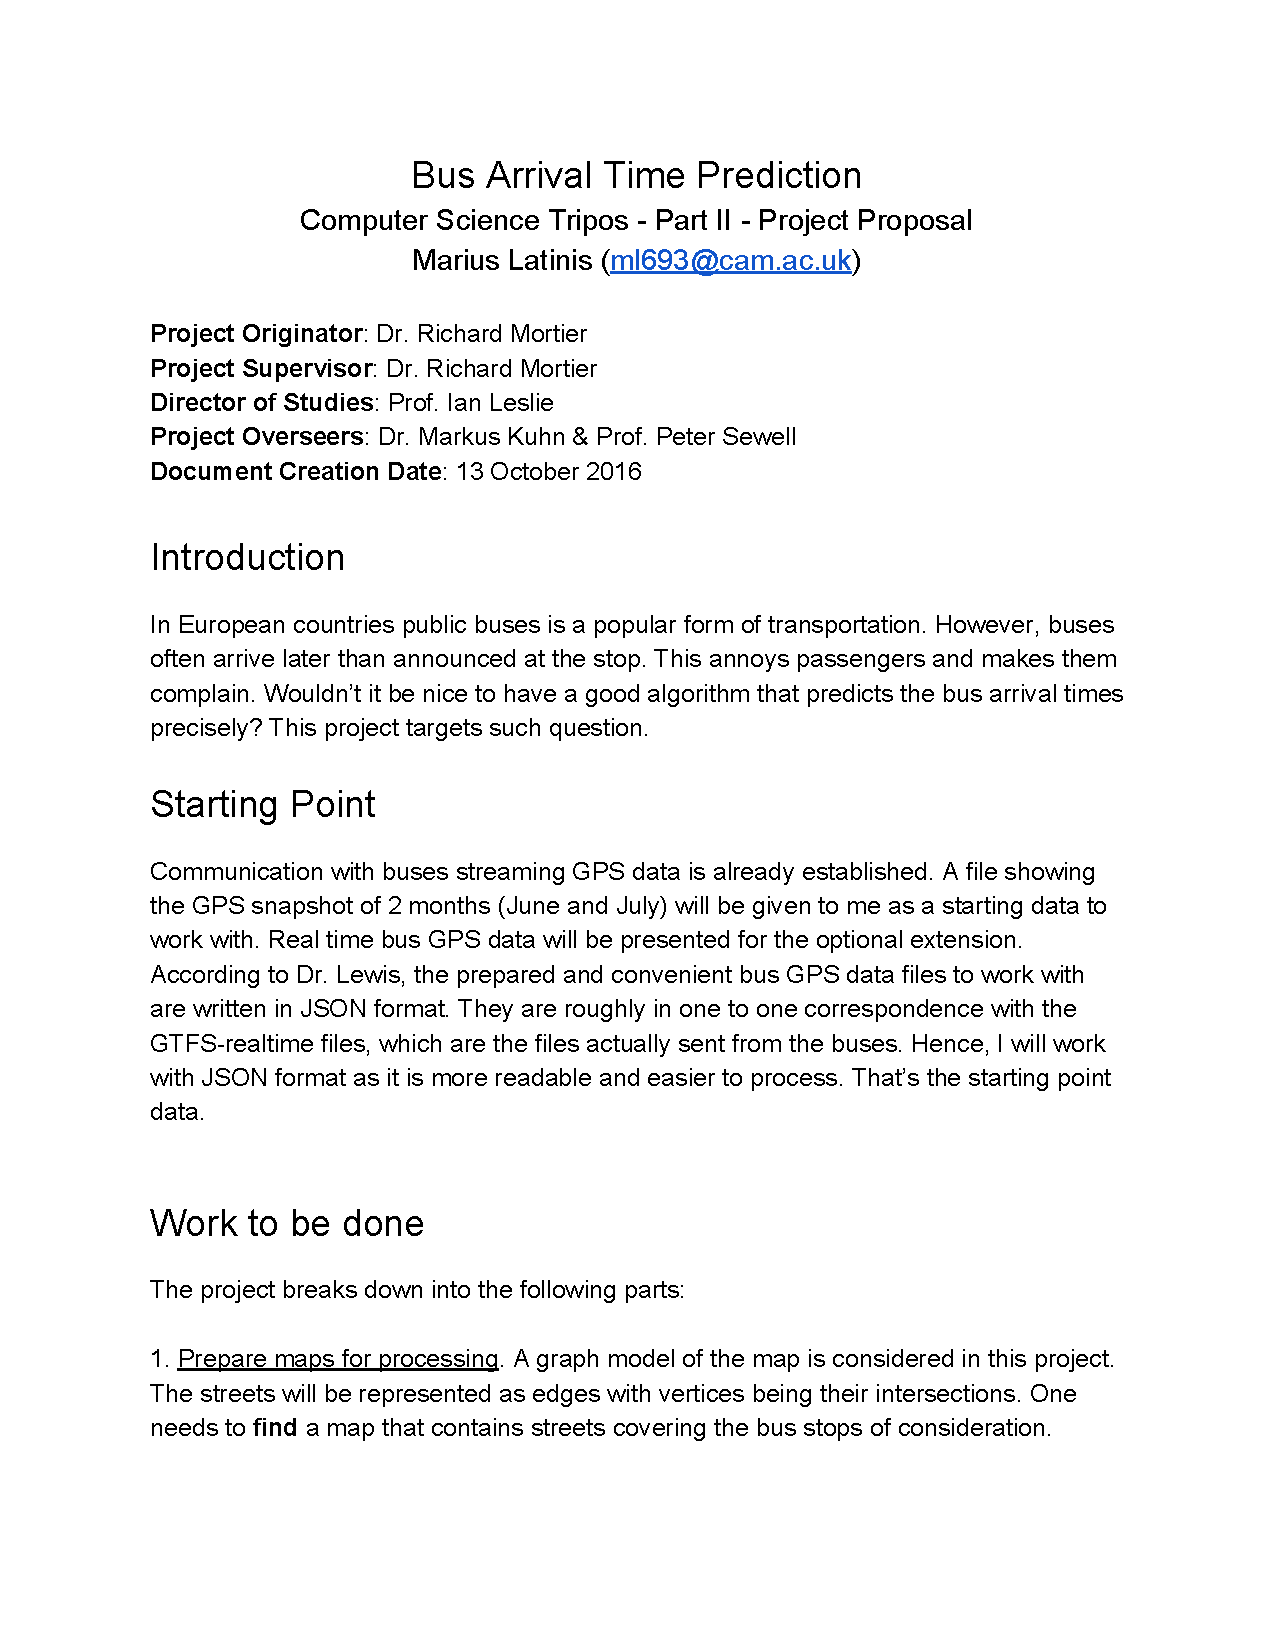
\includepdf[pages=-]{proposal.pdf}

\end{document}
